\documentclass[preview]{standalone}
\usepackage{tikz}
\usetikzlibrary{backgrounds,shapes.arrows}

\begin{document}
    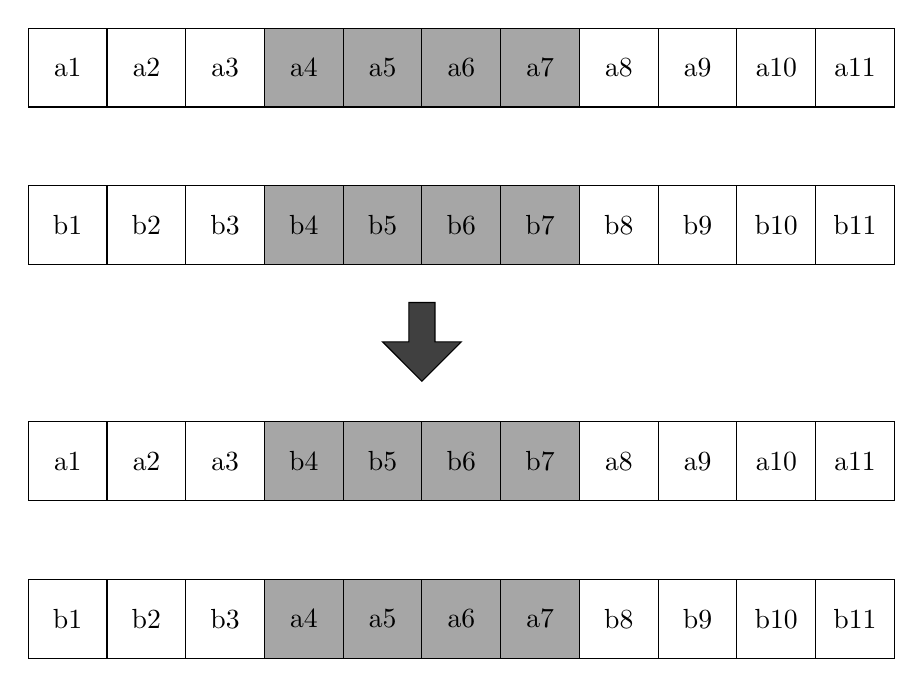
\begin{tikzpicture}[
    every node/.style={draw, shape=rectangle, minimum size=1cm}
    ]
    
    \begin{scope}
    \path foreach \i in {1,2,...,11}
      {(\i,2) node{a\i}};
    \path foreach \i in {1,2,...,11}
      {(\i,0) node{b\i}};
    
    \begin{scope}[on background layer, shift={(-0.5,-0.5)}]
       \foreach \i in {4,...,7} 
         \fill[gray!70](\i, 2) rectangle +(1,1)
               (\i, 0) rectangle +(1,1);
    \end{scope}
    \end{scope}
    
    \path (5.5, -1.4) node[single arrow,fill=black!75,shape border rotate=270]{};
    
    \begin{scope}[yshift=-5cm]
    \path foreach \i in {1,2,3,8,9,10,11}
      {(\i,2) node{a\i}};
    \path foreach \i in {4,5,6,7}
      {(\i,2) node{b\i}};
    \path foreach \i in {1,2,3,8,9,10,11}
      {(\i,0) node{b\i}};
    \path foreach \i in {4,5,6,7}
      {(\i,0) node{a\i}};
      
    \begin{scope}[on background layer, shift={(-0.5,-0.5)}]
       \foreach \i in {4,...,7} 
         \fill[gray!70](\i, 2) rectangle +(1,1)
               (\i, 0) rectangle +(1,1);
    \end{scope}
        
    \end{scope}

    

    \end{tikzpicture}
\end{document}
